\documentclass[10pt]{article}

\usepackage{amsmath}
\usepackage{fullpage}
\usepackage{array}
\usepackage{graphicx}
\usepackage{gensymb}
\usepackage{booktabs}
\usepackage{gensymb}
\usepackage{graphicx}

\graphicspath{ {../Images/} }

\date{2014-6-22}
\pagestyle{empty}
\setlength{\parindent}{0pt}

\begin{document}
\begin{center}
\begin{Large}\textbf{Physical Science 303 - Activity}\end{Large} \\
\smallskip
%\begin{large} Acceleration \end{large}
\end{center}
%%%%%%%

\section{Finding the coefficient of friction}
\subsection{Review}
We first review the different types of frictional forces.
\begin{enumerate}
\item Static frictional force: the frictional forces acting on the bodies at rest but subjected to certain external forces.  The direction is opposite to the tendency of the relative motion.  The magnitude is given by
  \begin{equation}
    |\vec{F}| = \mu_{s}N
  \end{equation}
where $\mu_s$ is the coefficient of static friction and $N$ is the normal force. 
\item Kinetic frictional force: the frictionl force acting on the bodies in motion.  The direction is opposite to that of the relative motion.  The manitude is given by
  \begin{equation}
    |\vec{F}| = \mu_{k}N
  \end{equation}
\end{enumerate}
Experimentally $\mu_s>\mu_k$.  
\subsection{Activity}
\begin{enumerate}
\item \textbf{Required Box}: Box 1
\item \textbf{Required Items}: 5N Pull Springs, Thread Spool, Friction Box, Super Pulley
\end{enumerate}
\begin{enumerate}
\item Prepare the setup as shown in the figure \ref{pulleyfri}.
\begin{figure}[h]
\label{pulleyfri}
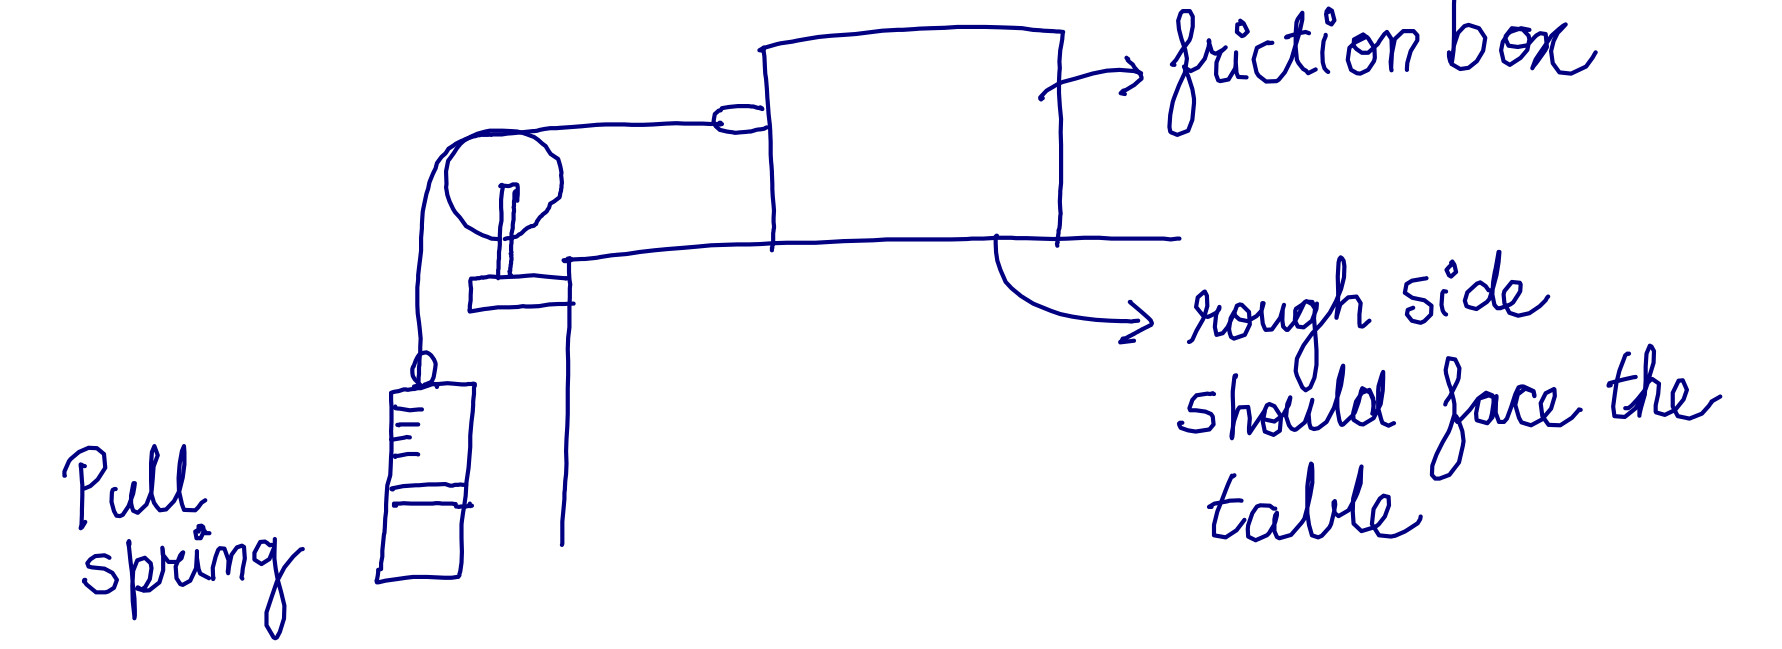
\includegraphics[scale=.5]{pulleyfric}
\centering
\caption{Setup}
\end{figure}
\item Gradually start pulling the pull spring till the friction box just starts moving.
\item Observe and note the reading in the pull spring.  \emph{Make sure to write appropriate units.}\\
Force:\underline{\hspace{5cm}}
\item Finally using the pull spring, weight the friction box and write down with appropriate units.\\  Weight:\underline{\hspace{5cm}}
\end{enumerate}
\subsection{Theoretical Analysis}
In this section we aim to find the coefficient of static friction.
\begin{enumerate}
\item Draw the free body diagram corresponding to the friction box and the pulley with string (essentially you just need to show tension for the pulley).  Use the generic labels for the forces and tension.
\vspace{250px}
\item In the experiment, you observed the force for which the box \emph{just} starts moving.  Does is correspond to the static or kinetic friction?  
\vspace{50px}
\item Using the appropriate formula for the friction and observed values (force and weight), compute the coefficient of friction.
\vspace{250px}  
\end{enumerate}
Answer the following questions
\begin{enumerate}
\item If you increase the weight of the friction box, will the coefficient of friction change?  Why or why not?
\vspace{100px}
\item Is the experimental value of the coefficient of kinetic friction exactly equal to the theoretical value?  Why not? List three reasons.
\end{enumerate}

\end{document}
